  \subsection{Figura de Lissajous}
               
      La figura de Lissajous, son comúnmente usadas para la determinación de la diferencia
      de fase entre dos señales de la misma frecuencia. Los osciloscopios cuentan con un modo
      conocido como \textbf{modo X-Y}, el cual toma una de las señales y la inyecta en el canal
      Y, y la otra en el canal X de esa manera, internamente el osciloscopio se encarga de 
      sumar punto a punto las señales y muestra en pantalla la figura de Lissajous formada por
      dichas señales.

         \begin{figure}[H]
            \centering
            \frame{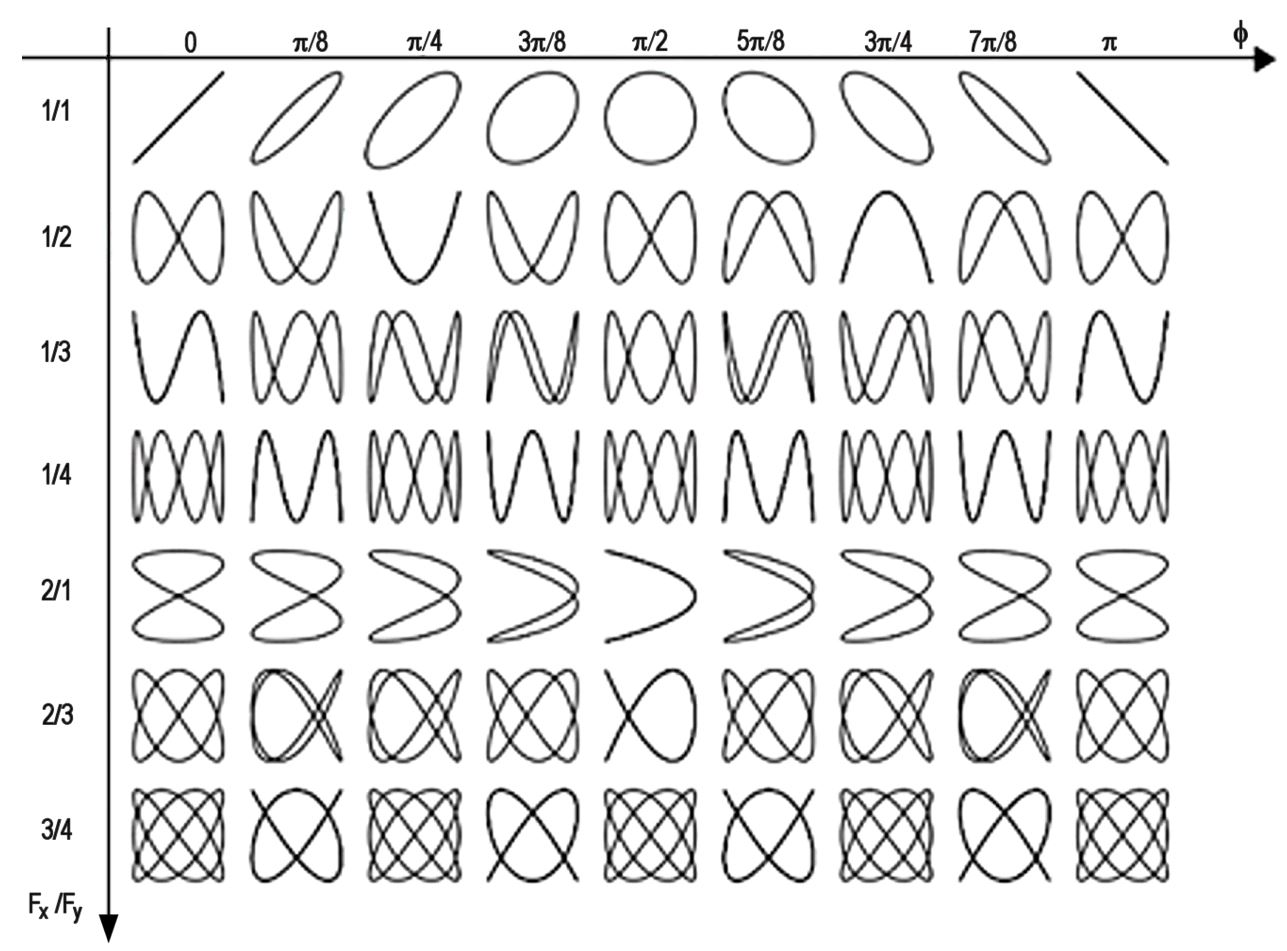
\includegraphics[width=.7 \textwidth]{Imagenes/MarcoTeorico/LissajousFiguras.jpg}}
            \caption{Figuras de Lissajous.}
            \label{fig:LissajTipos}                 
         \end{figure}

      De los tipos de figuras de Lissajous vistas en la Figura \ref{fig:LissajTipos}, 
      en el presente trabajo practico, se destacara las figuras de \textbf{tipo elípticas}, 
      las cuales son formadas por señales con valores de fase relativamente distinto a $\pi$/2 
      y con diferentes amplitudes

      \begin{figure}[H]
         \centering
         \frame{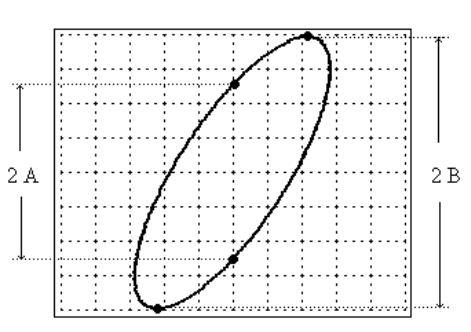
\includegraphics[width=.5 \textwidth]{Imagenes/MarcoTeorico/LissajousEliptico.png}}
         \caption{Figura de Lissajous de tipo elíptico.}
         \label{fig:LissajElip}           
      \end{figure}

      La obtención de la diferencia de fase entre las señales se pueden determinar de la
      siguiente manera.
      \newpage

      \noindent Considerando las siguientes expresiones
      \begin{align}
         x &= A\cdot \sin(\omega t) \hspace{10pt} ; \hspace{10pt} y = B\cdot \sin(\omega t + \phi) \ , \notag
      \end{align}
      
      \noindent de la Figura \ref{fig:LissajElip} se deduce que cuando
      \begin{align}
         x &= 0 \hspace{10pt} , entonces \hspace{10pt} y = A \ , \notag
      \end{align}   

      \noindent lo cual se repetirá cuando \(\omega\) t = 0, 2\(\pi\), .... n\(\pi\). Finalmente para 
      \( \omega \) t = 0 se obtiene

      \begin{align}
         \hspace{20pt} y &= B\cdot \sin(\phi) = A \hspace{20pt} \therefore \hspace{-70pt} \Aboxed{\dfrac{A}{B} = \sin(\phi)} \ . \notag 
      \end{align}
      
      \noindent De la última ecuación despejamos el ángulo de desfase
      \begin{equation}
         \boxed{\varphi = \sin^{-1}\ \left(\dfrac{A}{B} \right)}   \ . \label{eqn:AngDeDesf}   
      \end{equation}

